\chapter{日本地区机器学习方法预估震级效果}
\section{数据分析与预处理}
\indent 利用第二、三章所描述的方法,本文搭建并实现了$\tau_{c}$方法和机器学习类模型进行效果检验。考虑到震级紧急预估的应用场景和所需要的基础设施需求,我们将研究区域定位日本主岛区域附近。考虑到地震紧急预估的时效性,选取地震事件距离台站为1个相对经纬距离(约100km)内的记录。原始全数据集使用了日本KIK和KNET两台站网从2015至2017年所记录到的所有大于3级且震源靠近日本岛主体的地震记录,除此之外并无经过其他任何的主动事件挑选,事件分布如下图4.1所示。\\
\begin{figure}[!h] 
\centering 
 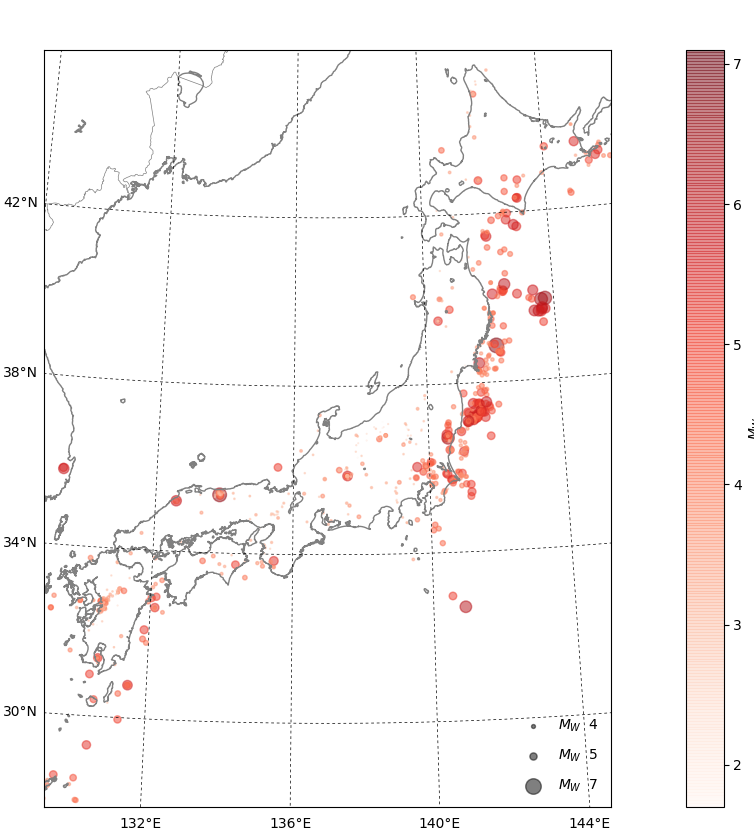
\includegraphics[width=0.9\linewidth]{img/basemap.jpg} 
 \renewcommand{\figurename}{图} 
\caption{全数据集地震事件} 
%英文标题begin 
\addtocounter{figure}{-1} \vspace{-5pt} 
%\SetEnglishCaption 
\renewcommand{\figurename}{Fig} 
\caption{Full data set earthquake event} 
\renewcommand{\figurename}{图} 
%英文标题end 
\label{fig:network-device-influence.png} 
\end{figure}
\indent 原始全数据中共包含了840个地震事件,合计50314条记录,具体的分布和统计如下图4.2和4.3所示,其中包含了3级至4级地震事件共420个、10145条地震台站记录,4级至5级地震事件共216个、14629条地震台站记录,5级至6级地震事件共61个、10740条地震台站记录,6级以上地震事件共8个、1004条地震台站记录。地震事件的分布特点如图4.2(b)所示存在很严重左偏,这种不均分布特征对机器学习模型训练带来一些阻碍。\\
\begin{figure}[!h] 
\centering 
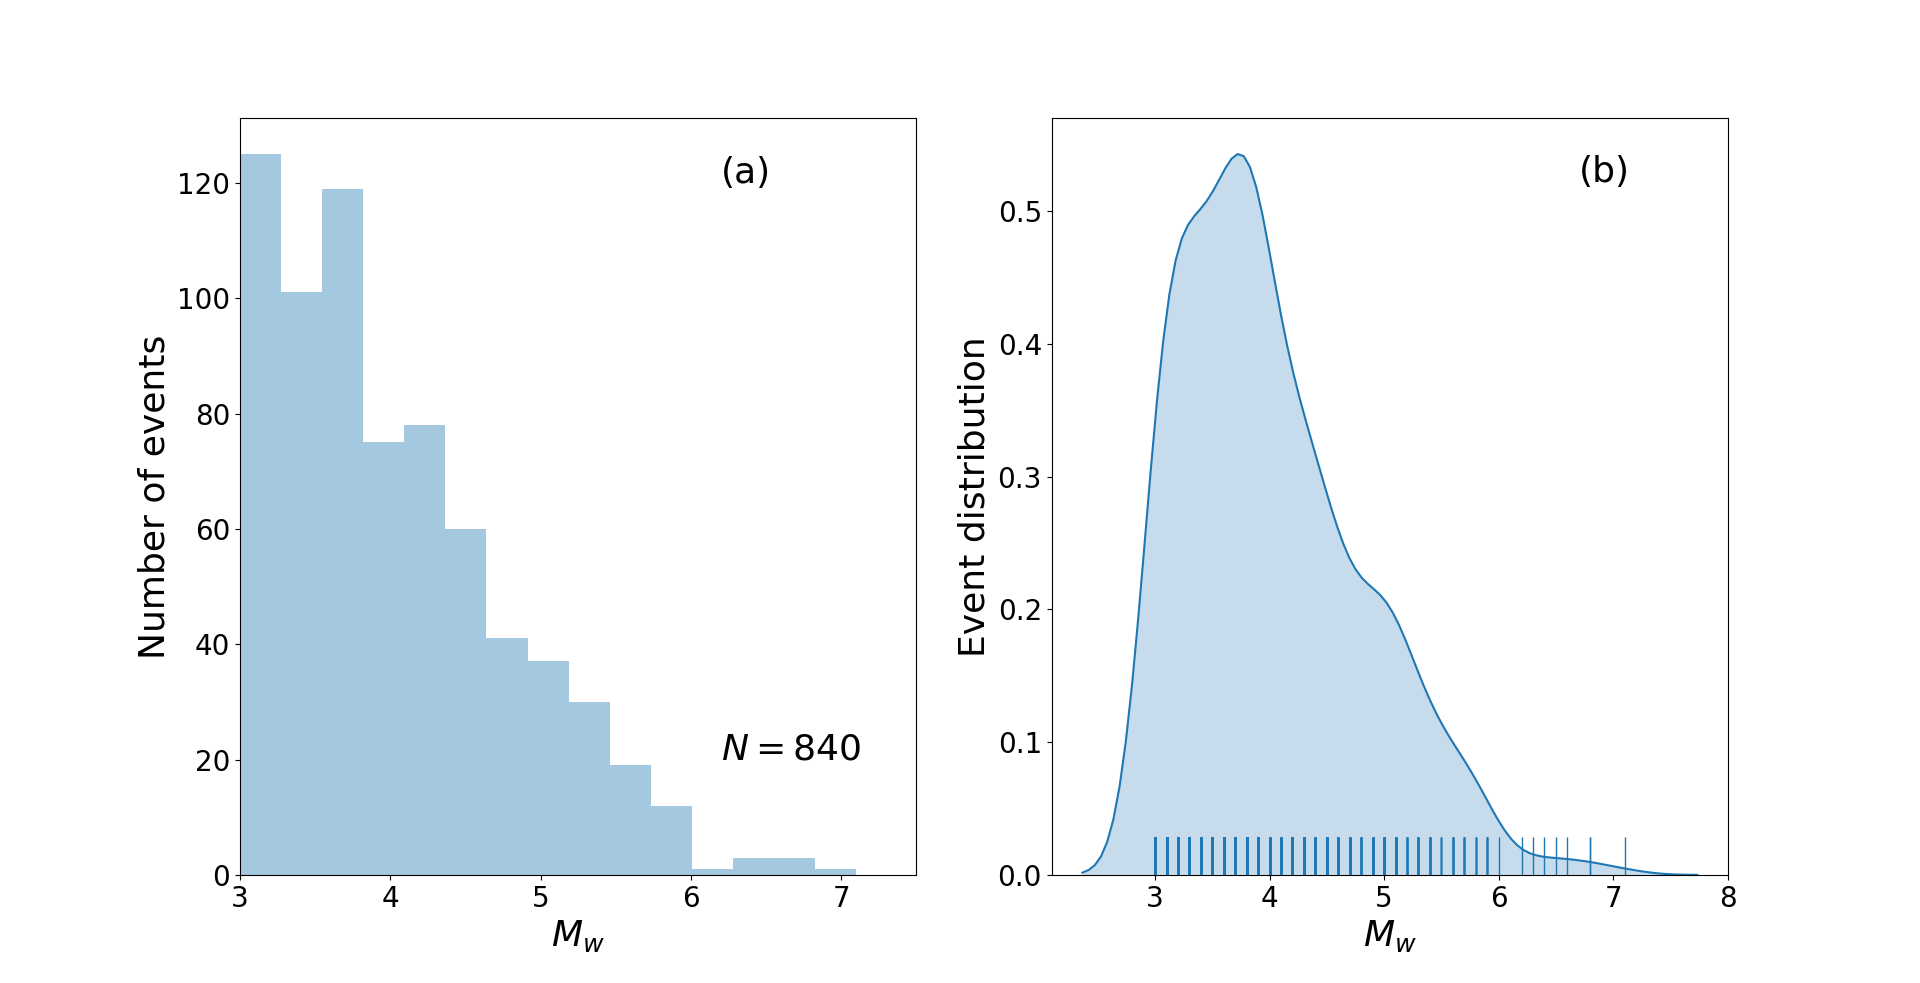
\includegraphics[width=0.95\linewidth]{img/Event_distribution.png}
\renewcommand{\figurename}{图} 
\caption{数据集中地震单条记录的震级分布。横轴为单条记录的震级$\mathbf{M}_{\mathbf{w}}$。\\
(a)图中纵轴为该震级的事件记录数目。(b)图中纵轴为单条记录震级大小分布的概率密度} 
%英文标题begin 
\addtocounter{figure}{-1} \vspace{-5pt} 
%\SetEnglishCaption 
\renewcommand{\figurename}{Fig} 
\caption{The magnitude distribution of a single earthquake record in the data set. The horizontal axis is the magnitude of a single record $\mathbf{M}_{\mathbf{w}}$. \\
(a) The vertical axis in the figure is the number of event records for this magnitude. (b) The vertical axis of the graph is the probability density of a single record magnitude distribution.
} 
\renewcommand{\figurename}{图} 
%英文标题end 
\label{fig:network-device-influence.png} 
\end{figure}
\indent 图4.3(a)显示了以单一记录为视角的不同震级记录数目的分布。虽然一次地震事件中对于大地震的台站记录数量多于小地震,这使得不同级别地震发生频率上不均衡导致数据不均衡的问题得到一定程度上的缓解,但震级分布总体来看仍然不够均匀,小地震记录条数远远多于大地震。客观上大地震释放的能量巨大,如若不能良好处置则会给人们正常生活生产带来了严重破坏和致命打击,所以大地震往往是紧急预警系统中容错率较低的部分,人们并不希望地震预警系统对于来临大地震没有正确的响应。但从数据量的角度来看大地震出现频率低,可供机器学习模型学习的信息量少,这不利于模型采集到关于如何预估大型地震的规则,给模型的训练带来较大的困扰。\\
\indent 对于类别不均衡,现有的技术大体上有三类做法(周志华,2016):第一类是对训练集里的正类样本(大地震事件)进行过采样,即通过增加正列数量使得在训练集中、反列样本(大地震事件、小地震事件)数量差距变小。第二类与第一类方法相反,采取对负样本欠采样的方式平衡有偏分布类别。第三类方法为直接对原训练集进行学习,但对训练好的模型评判阈值进行平移,改变评判标准。采取第二种欠采样的方式会丢失很多反例,使得训练集数据量变少,在训练数据有限的情况下并不适用。第三类方法更多的应用于分类问题,不同于我们所设计回归问题。综上我们采取在训练集中对大地震数据过采样再加一定噪音的方法增广正例样本,以此处理数据分布不平衡问题。将原始的如图4.3(a)分布修正为图4.3(b),一定程度上缓解分布不均带来的训练问题。\\
\begin{figure}[!h] 
\centering 
 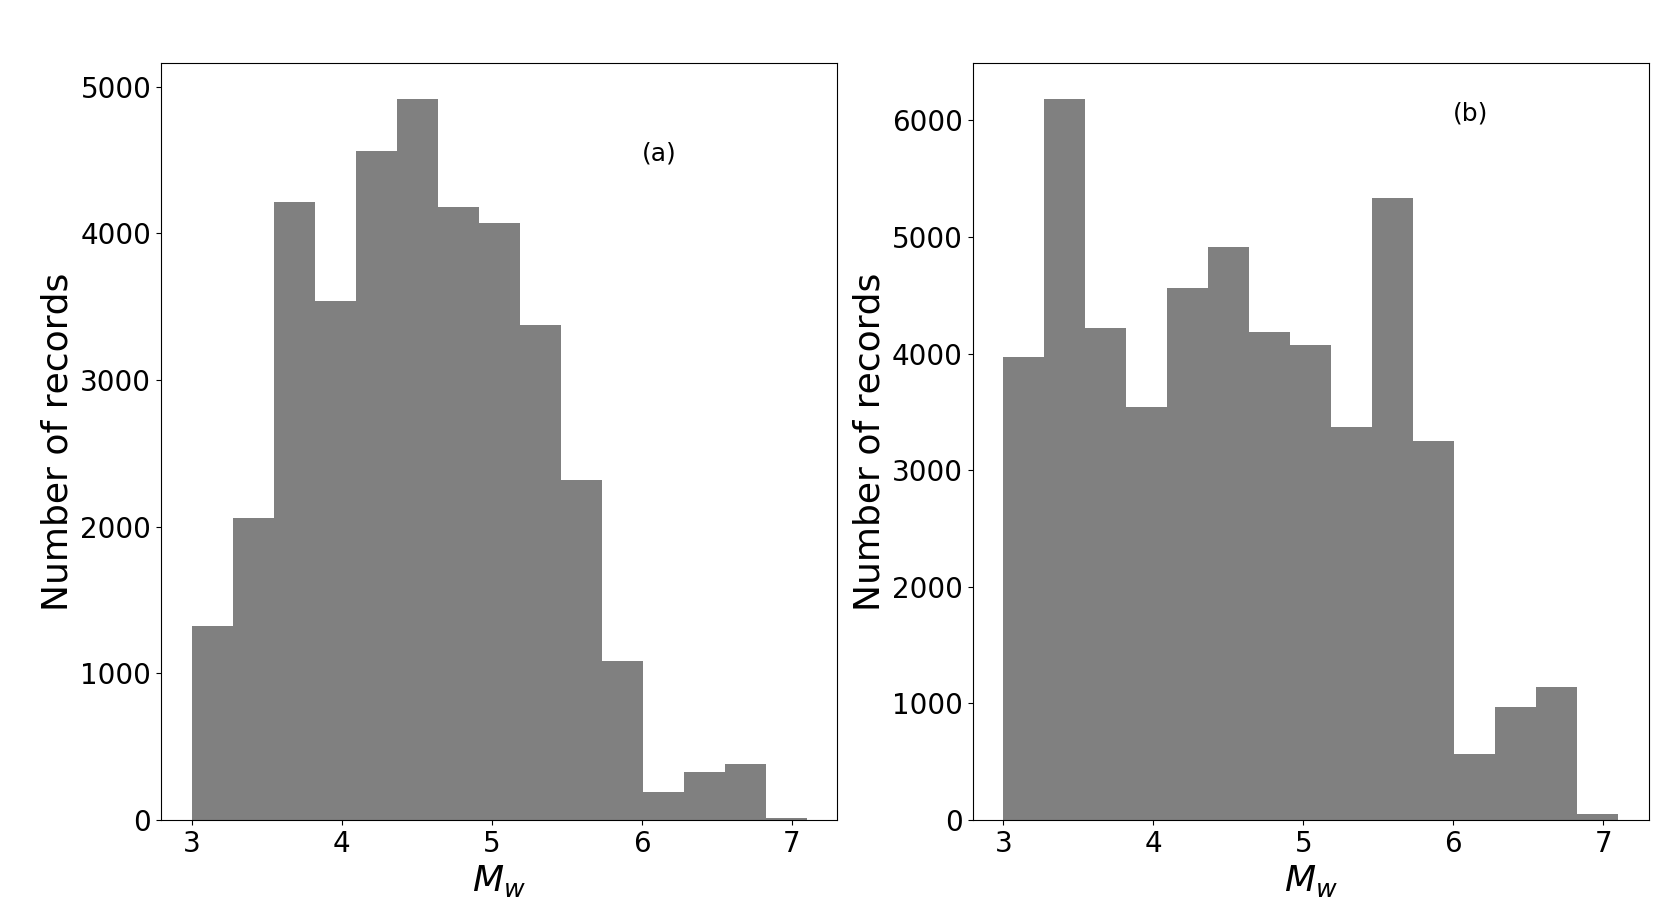
\includegraphics[width=0.95\linewidth]{img/event_dist.png} 
 \renewcommand{\figurename}{图} 
\caption{数据集中地震记录的震级分布。横轴为震级$\mathbf{M}_{\mathbf{w}}$,纵轴为该震级的台站记录数目。\\
(a) 原始分布;(b) 调整后分布} 
%英文标题begin 
\addtocounter{figure}{-1} \vspace{-5pt} 
%\SetEnglishCaption 
\renewcommand{\figurename}{Fig} 
\caption{Magnitude distribution of seismic records in data sets, The horizontal axis is the magnitude $\mathbf{M}_{\mathbf{w}}$, and the vertical axis is the number of stations recorded for this magnitude.\\
(a) Original distribution; (b) Adjusted distribution} 
\renewcommand{\figurename}{图} 
%英文标题end 
\label{fig:network-device-influence.png} 
\end{figure}


\section{机器学习类模型与传统模型的比较}
\subsection{NN震级预估模型的效果评估与比较}
\indent 训练曲线如图4.4所示,图中两条图线分别代表了训练集和交叉验证集的均方根误差(RMSE)随着训练步数的变化。NN模型在经过大约15000个步训练步长后,达到此模型结构下的最佳权值状态。超过15000个训练步长后后虽然训练数据集级上模型表现持续变好,但在交叉检验数据集上RMSE停止减小并开始增大,说明模型已经进入第3章所描述的过拟合状态,此时再增加训练轮数只会让模型更加过拟合拥有更差的。故当完成15000个训练步长时触发提前停止条件(Early Stopping),在此训练步数上停止训练并存储此时的模型最佳权值。\\
\begin{figure}[!h] 
\centering 
 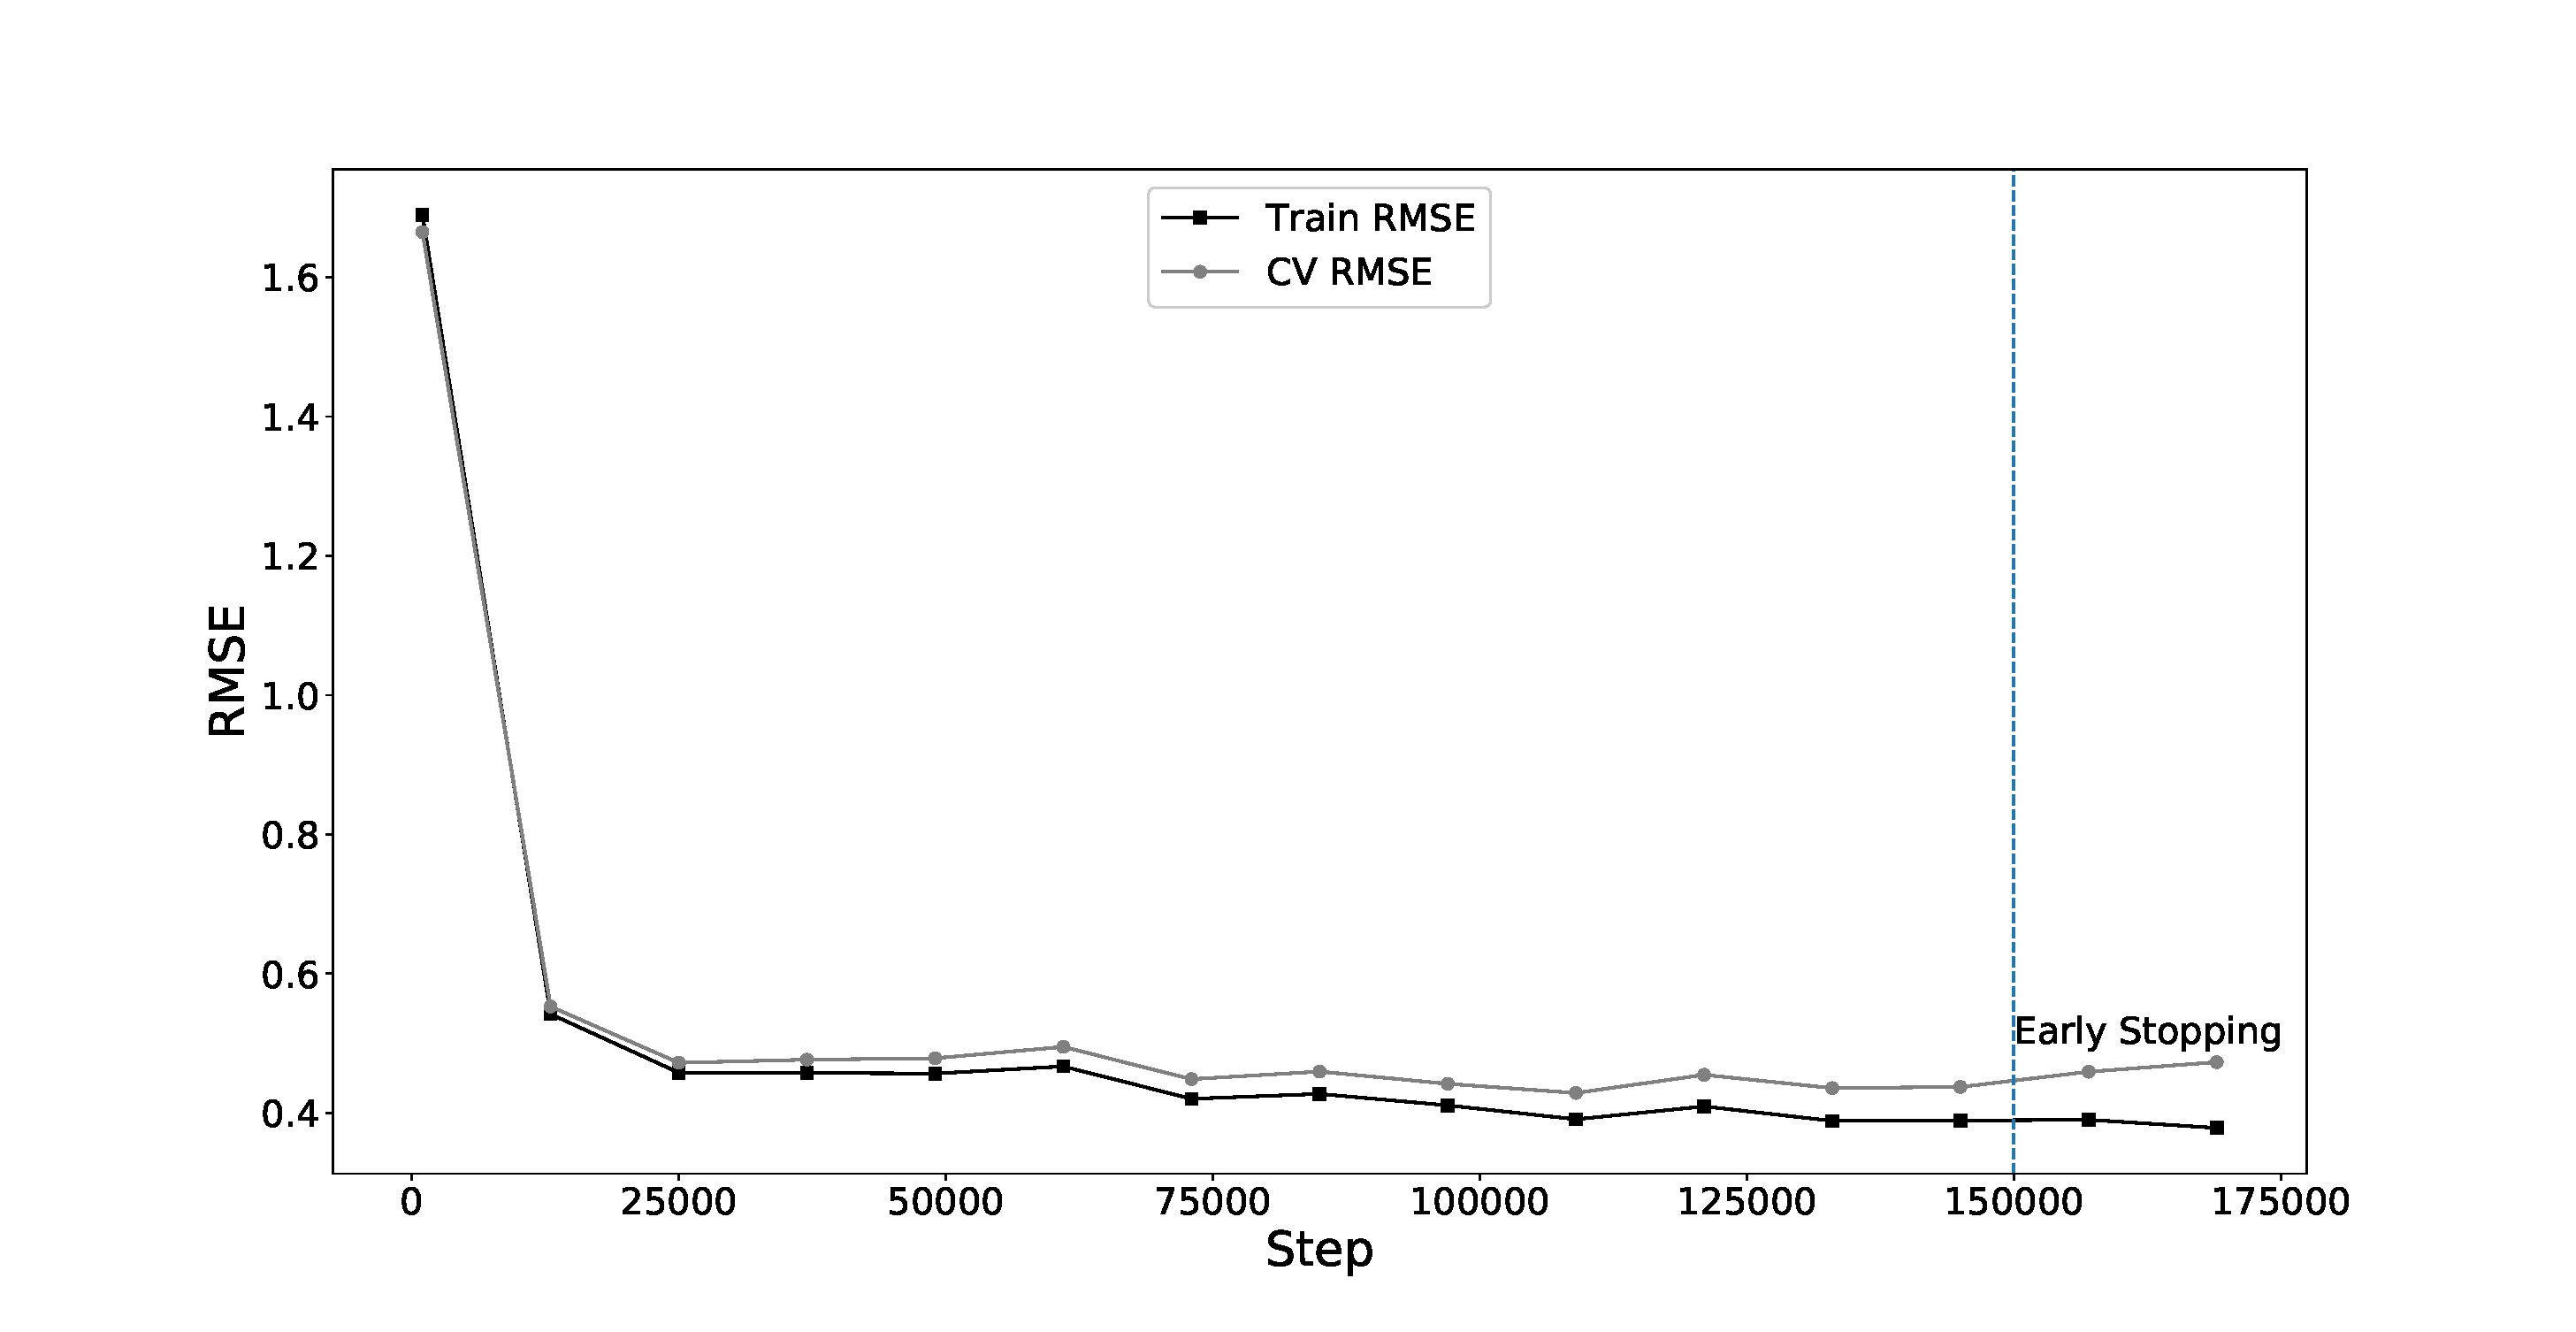
\includegraphics[width=0.9\linewidth]{img/6.eps} 
 \renewcommand{\figurename}{图} 
\caption{NN模型训练曲线。横轴为训练步数,纵轴为均方根误差(RMSE)。} 
%英文标题begin 
\addtocounter{figure}{-1} \vspace{-5pt} 
%\SetEnglishCaption 
\renewcommand{\figurename}{Fig} 
\caption{NN Model training curve. The horizontal axis is the number of training steps and the vertical axis is the root mean square error (RMSE).} 
\renewcommand{\figurename}{图} 
%英文标题end 
\label{fig:network-device-influence.png} 
\end{figure}
\indent 在图4.5和4.6中我们还原Kanamori (2008)的$\tau_{\mathrm{c}}$方法(以下简称为“K方法”),并使其与NN模型在同样的测试数据集上相比较。图4.5(a) K方法的结果中的实线为拟合$\tau_{\mathrm{c}}$和$\mathrm{M}_{\mathrm{w}}$的线性关系,实线上下两条虚线代表了一个平均标准差的范围。值得注意的是在Kanamori (2008)中一共使用了来自3个地区共54个事件的集合对$\tau_{\mathrm{c}}$和$\mathrm{M}_{\mathrm{w}}$的线性拟合。每个事件的$\tau_{\mathrm{c}}$值都定义为离震中最近的4个台站$\tau_{\mathrm{c}}$的平均值。这与本文定义略有出入,本文中$\tau_{\mathrm{c}}$值定义为距离震中100km内的所有台站的平均值。\\
\indent 同时K方法中没有进行数据集的分割,其中线性回归模型所使用的训练集和测试集都为同一数据集,即先使用全54个地震事件进行回归模型训练,然后又在这54个事件上进行误差计算。这使得K方法在模型评估效果上存在一定的隐患。在本文的研究实验中所有方法的效果评估都严格按照第3章中所叙述的数据集分割方式进行。\\
\indent 如图4.5所示当NN模型与和K方法(2008)考察相同震级范围,都研究震级大于4级的事件区间并以地震事件震级预估误差作为评判。图中的小正方形为多台站联合预估震级的平均结果,而方框上下的延长线为该事件的一个标准差的置信区间。结果显示出NN模型和K方法对于单一地震事件在测试集上的方均根误差别为0.29和0.59。相比于K模型体现出性能明显优势,NN模型预估震级误差更小约为K方法的一半。直观来看在图4.5中NN模型的(a)图相比于K模型的(b)图斜率更大,意味着对于同一特征NN模型有着更强的分辨率。\\
\begin{figure}[!h] 
\centering 
\includegraphics[width=\linewidth]{img/7.eps} 
\renewcommand{\figurename}{图} 
\caption{震级预估效果对比(最低截至震级为3级)。横轴为真实震级。\\
(a) 采用Kanamori et al. (2008)方法的结果,纵轴为K方法的$\log \left(\tau_{\mathrm{c}}\right)$;(b) NN模型的结果,纵轴为机器学习模型给出的预估震级} 
%英文标题begin 
\addtocounter{figure}{-1} \vspace{-5pt} 
%\SetEnglishCaption 
\renewcommand{\figurename}{Fig} 
\caption{Comparison of magnitude prediction effects (minimum to magnitude 3). The horizontal axis is the true magnitude.\\
(a) Using the results of Kanamori et al. (2008), the vertical axis is the $\log \left(\tau_{\mathrm{c}}\right)$ of the K method; (b) the result of the NN model, the vertical axis is the predicted magnitude given by the machine learning model.} 
\renewcommand{\figurename}{图} 
%英文标题end 
\label{fig:network-device-influence.png} 
\end{figure}
\indent 如果把研究范围的最小震级限制拓展至3级,按照图4.5的方法得到图4.6所示的结果。将3级至4级地震事件加入到考察范围内后,NN模型和K方法的预估能力都有明显下降。两方法的方均根误差分别升至0.51和1.06,这意味着两类模型对于一定程度的低级别地震震级的预估能力劣于中等级别的地震。\\
\begin{figure}[!h] 
\centering 
\includegraphics[width=\linewidth]{img/8.eps} 
\renewcommand{\figurename}{图} 
\caption{震级预估效果对比(最低截至震级为3级)。横纵坐标同图4.5。\\
(a) 采用Kanamori et al. (2008)方法的结果;(b) NN模型的结果} 
%英文标题begin 
\addtocounter{figure}{-1} \vspace{-5pt} 
%\SetEnglishCaption 
\renewcommand{\figurename}{Fig} 
\caption{Comparison of magnitude prediction effects (minimum to magnitude 3). The horizontal and vertical coordinates are the same as in Figure 4.5. \\
(a) Results using Kanamori et al. (2008) (b) The results of NN model} 
\renewcommand{\figurename}{图} 
%英文标题end 
\label{fig:network-device-influence.png} 
\end{figure}
\indent 图4.7两子图展示了NN方法和K方法对于不同震级的地震记录,只使用单一台站三分量信息的情况下进行预估的误差情况。整体而言在各个震级上K方法预估的表现虽然稳定但误差均大于NN方法。对所有地震的单台站预估平均误差中,NN方法效果最差误差最大出现在7级以上地震约为1.6级,K方法效果最好误差最小出现在6级地震但平均误差仍有1.1级。\\
\indent K方法中单台站的预测误差大小随着震级增加而略微减小。这种现象可能由于图4.8中所示的地震事件与台站记录数量分布随震级增加每个事件被记录到的台站数越多的特征。这种特征使得大型地震相对较小地震有更多数据记录,也就意味着K方法中使用$\left(\tau_{\mathrm{c}}\right)$平均值做震级预估时的特征时是更为无偏的估计,进而在以地震事件为视角做$\left(\tau_{\mathrm{c}}\right)$与$\mathbf{M}_{\mathbf{w}}$线性回归时得到参数能更好应用于较大型地震的震级预估。注意到图4.8考虑因6级以上地震发生频率低、数据量较少故并没有进行展示。\\
\indent 图4.7(a)为NN方法的误差分布分为蓝色和红色两个区域。中间的蓝色区域内单台站预估出的震级误差稳定,而两侧红色区域误差随震级有较大的变化。结合4.7(b)结果佐证了在蓝色区域内物理本质上较为容易进行震级预估,一方面4级至6级地震的被台站记录数量足够多。同时地震破裂过程时长适中,能在较好被P波初到后3s的时长台站数据估计出。另一方面从考虑由于NN方法为机器学习方法,其本身是解释能力很强的方法,但在两侧红色区域仍不能轻易得到好的预估结果。这从反面一定程度上说明了在两侧红色区域存在客观问题使得震级预估问题本身不易实现。对于左侧红色区域NN模型的表现与K模型相似,可以认为因为数据量导致的震级预估不准确对于两种方法都存在。而右端红色高误差区域,可能是因为高能量地震的破裂情况难以被P波初到后3s的数据解释。\\
\begin{figure}[!h] 
\centering 
\includegraphics[width=\linewidth]{img/eb.eps} 
\renewcommand{\figurename}{图} 
\caption{不同方法在只使用单台站信息下不同震级地震预估的误差情况\\
(a)NN方法对不同震级地震的预估误差。其中两侧红色区域为预估非稳定区域,中间蓝色区域为稳定区域(b)K方法法对不同震级地震的预估误差} 
%英文标题begin 
\addtocounter{figure}{-1} \vspace{-5pt} 
%\SetEnglishCaption 
\renewcommand{\figurename}{Fig} 
\caption{Errors of different magnitude earthquake predictions under different methods using only one station information\\
(a) Estimation error of NN methods for earthquakes of different magnitudes. The red area on both sides is the estimated unsteady area, the middle blue area is the stable area (b)K method method, the prediction error of earthquakes of different magnitudes} 
\renewcommand{\figurename}{图} 
%英文标题end 
\label{fig:network-device-influence.png} 
\end{figure}
\begin{figure}[!h] 
\centering 
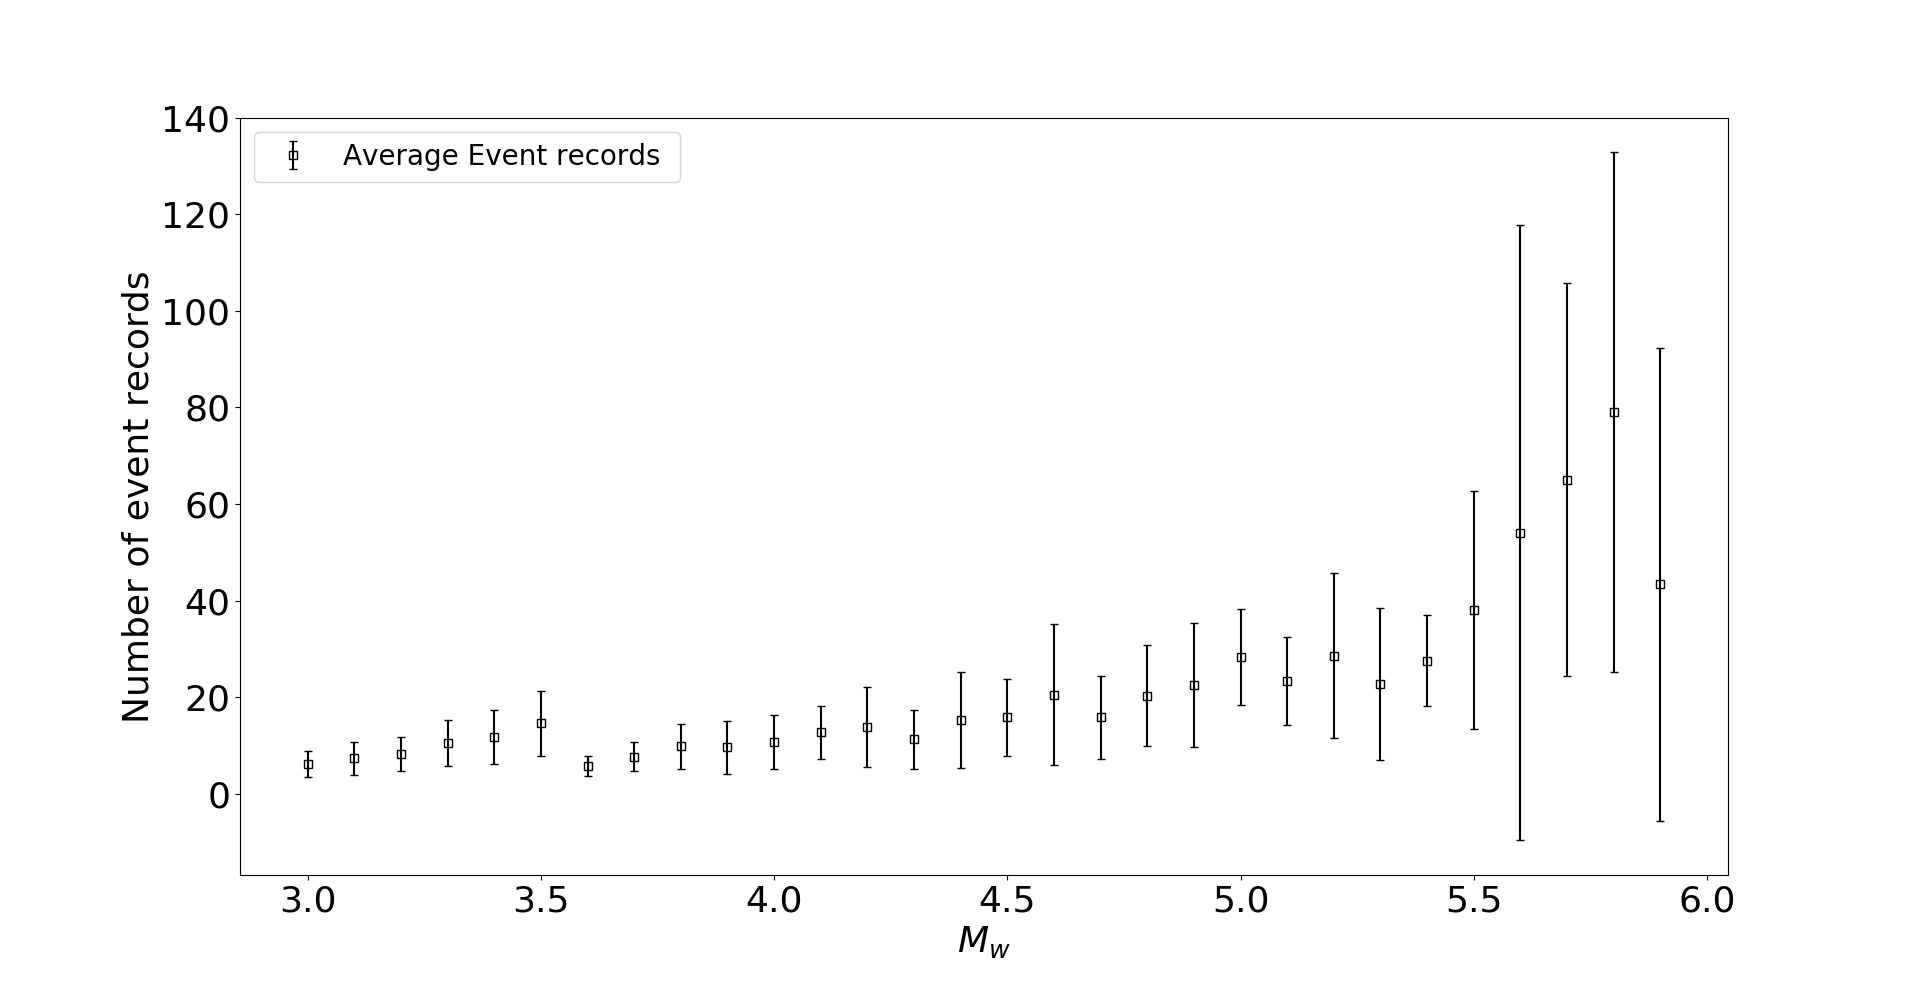
\includegraphics[width=\linewidth]{img/M-N.png} 
\renewcommand{\figurename}{图} 
\caption{数据集中地震事件与台站记录数量分布。横轴为事件震级$\mathbf{M}_{\mathbf{w}}$,纵轴为事件被记录到的数量} 
%英文标题begin 
\addtocounter{figure}{-1} \vspace{-5pt} 
%\SetEnglishCaption 
\renewcommand{\figurename}{Fig} 
\caption{The distribution of seismic events and station records in the data set. The horizontal axis is the event magnitude $\mathbf{M}_{\mathbf{w}}$, and the vertical axis is the number of events recorded.} 
\renewcommand{\figurename}{图} 
%英文标题end 
\label{fig:network-device-influence.png} 
\end{figure}
\indent 图4.9展示了K方法与NN方法以地震事件为视角震级预估的稳定性情况,图4的两个子图是在设置不同最低截至震级下预估误差方差的分布。可以看出在两种情形下,NN模型预估震级误差的总方差都更小展现出稳定的表现。并且从震级预估的方差分布特点来看,NN模型在两种最低截至震级情形下都展现出左移且高峰度的特点。综合来看NN模型的稳定性优于Kanamori(2008)的$\tau_{\mathrm{c}}$方法。\\
\begin{figure}[!h] 
\centering 
 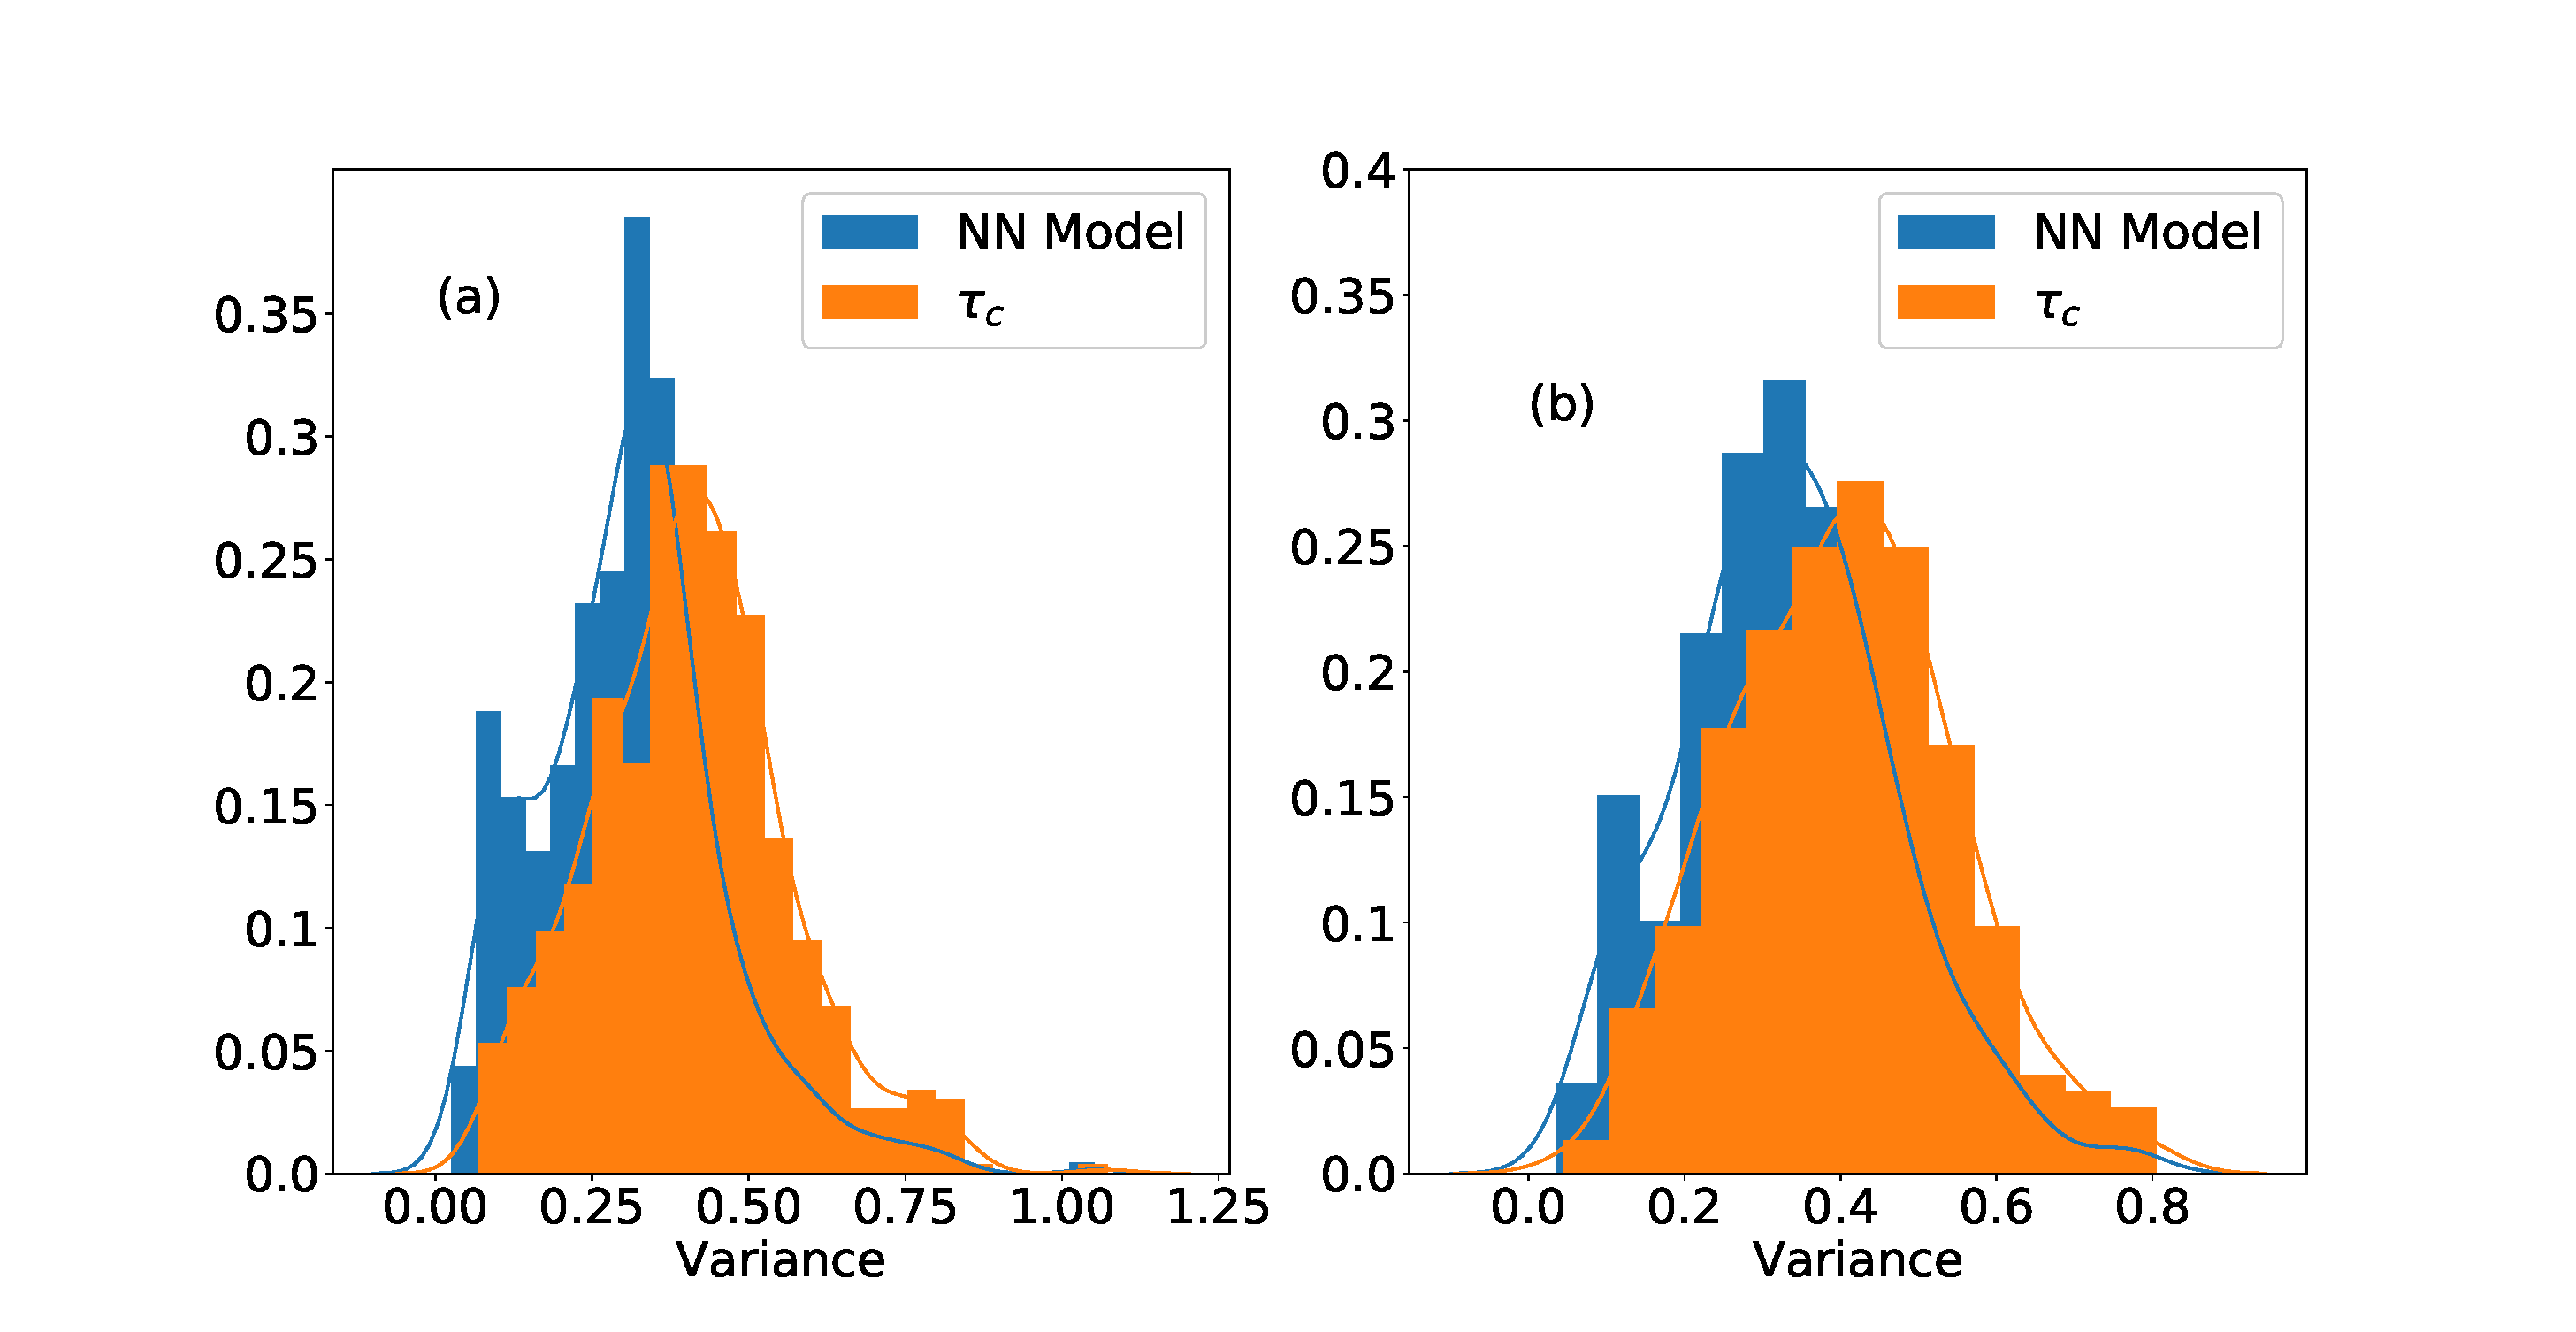
\includegraphics[width=\linewidth]{img/9.eps} 
 \renewcommand{\figurename}{图} 
\caption{单一事件预估方差分布。横轴为方差大小,纵轴为该方差的密度。\\
(a) 截至震级为4级K方法与NN模型方差分布;\\
(b) 截至震级为3级K方法与NN模型方差分布\\
} 
%英文标题begin 
\addtocounter{figure}{-1} \vspace{-5pt} 
%\SetEnglishCaption 
\renewcommand{\figurename}{Fig} 
\caption{Single event estimation variance distribution. The horizontal axis is the variance and the vertical axis is the density of the variance.\\
(a) The Kanamori method and the NN model variance distribution up to the
magnitude 4; \\
(b) The Kanamori method and the NN model variancedistribution up to the magnitude 3} 
\renewcommand{\figurename}{图} 
%英文标题end 
\label{fig:network-device-influence.png} 
\end{figure}


\subsection{CNN震级预估模型的效果评估与比较}
\indent 跟据3.3.2中所设计的CNN震级预估模型,本文搭建并完成了相应深度学习神经网络。由于计算机性能限制本模型只使用了全数据集50\%的数据量进行模型训练与评估。将训练好的模型在预设的验证集进行效果评估如图4.10和图4.11所示。其中图4.10展示了对于不同震级的地震记录,只使用单一台站信息的情况下进行预估的误差情况。在图中存在三种颜色区域,其中红色仍未震级预估不稳定区域,相比于NN模型的结果其中4到6级的预估效果仍然稳定并且在3.5到4级之间的绿色区域由NN模型的不稳定红色区域变为稳定区域。\\
\begin{figure}[!h] 
\centering 
 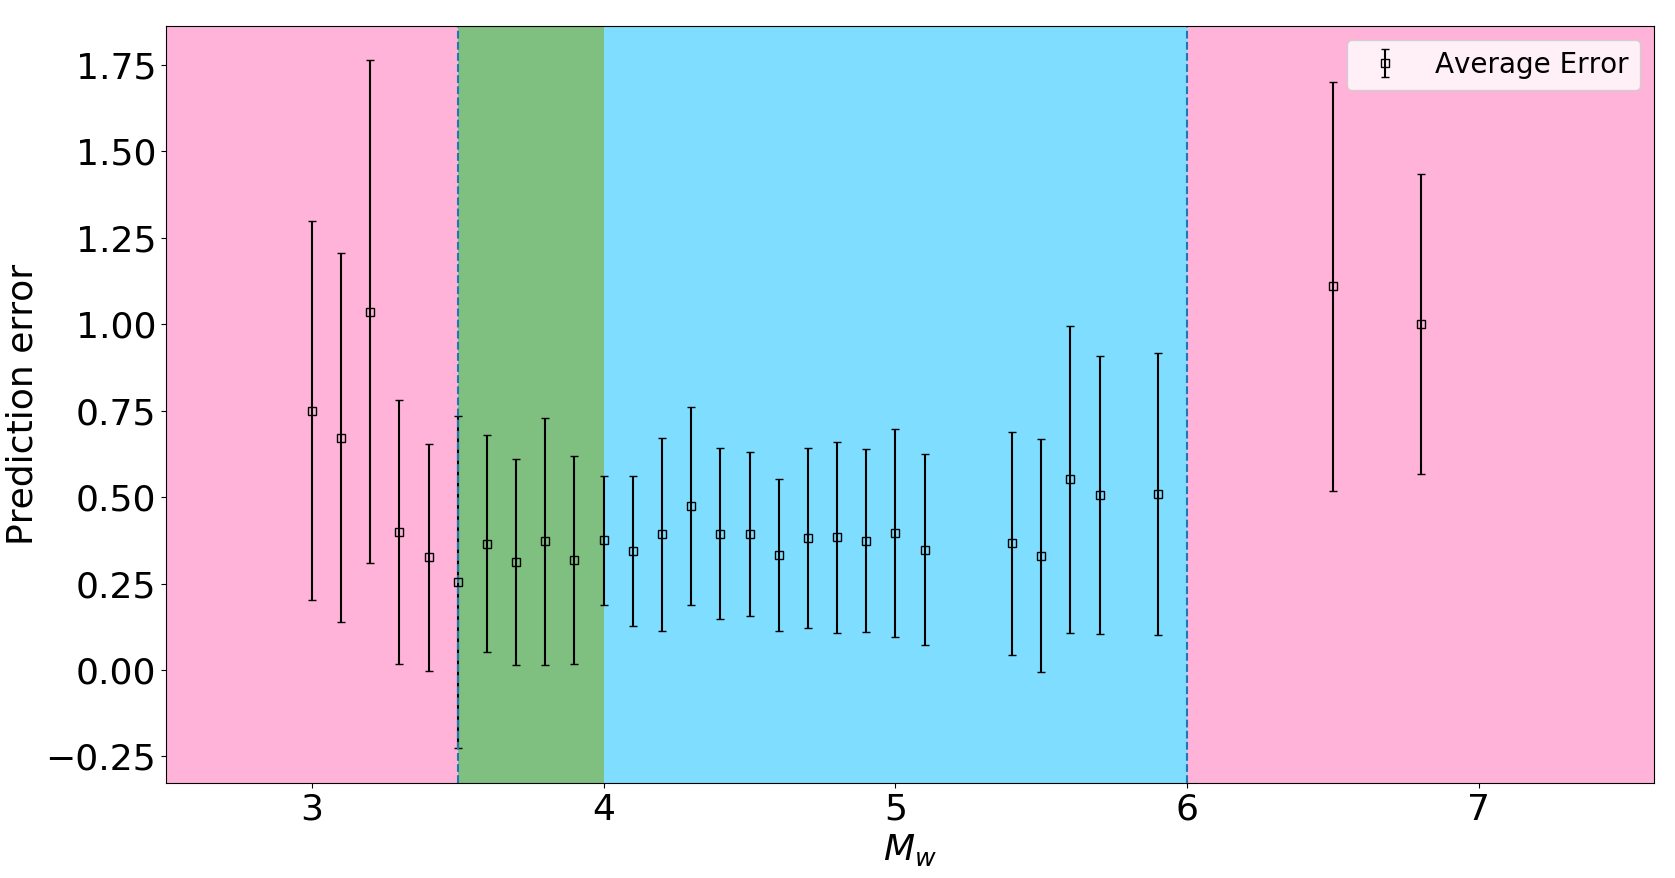
\includegraphics[width=\linewidth]{img/eb1_cnn.png} 
 \renewcommand{\figurename}{图} 
\caption{CNN震级预估模型单一台站记录的误差分布} 
%英文标题begin 
\addtocounter{figure}{-1} \vspace{-5pt} 
%\SetEnglishCaption 
\renewcommand{\figurename}{Fig} 
\caption{Error Distribution of Single Station Record in CNN Magnitude Estimation Model} 
\renewcommand{\figurename}{图} 
%英文标题end 
\label{fig:network-device-influence.png} 
\end{figure}
\begin{figure}[!h] 
\centering 
 \includegraphics[width=\linewidth]{img/CNN-PRE.eps} 
 \renewcommand{\figurename}{图} 
\caption{CNN模型震级预估效果\\
(a)最低截至震级为3级(b)最低截至震级为4级} 
%英文标题begin 
\addtocounter{figure}{-1} \vspace{-5pt} 
%\SetEnglishCaption 
\renewcommand{\figurename}{Fig} 
\caption{CNN model magnitude prediction effect\\
(a) Minimum cut-off magnitude is 3 (b) Minimum cut-off magnitude is 4} 
\renewcommand{\figurename}{图} 
%英文标题end 
\label{fig:network-device-influence.png} 
\end{figure}
\subsection{机器学习模型处理低信噪比的效果}
\indent 现实生活中当一次特大地震主震结束后,往往会伴随许多危害巨大的余震序列。虽然这些余震震级相对于主震来说都是较小的,但因建筑物、矿区等各种设施在主震来临时其已经结构遭受一定程度上的破坏,余震的发生往往会进一步破坏本来已经处于危险状况的设施结构,引发进一步的人员伤亡、加剧生产资料损毁,并且有可能引发次生的其他各种灾害。因此,余震震级的紧急预估具有十分重要的研究意义。\\
\indent 但令人遗憾的是传统震级预估方法在面对余震记录时并不能够准备的给出震级预估,低信噪比数据使传统方法在一定程度上趋于无效。而本文中所涉及的两类机器学习类震级预估方法,在处理低信噪比数据是都有着优秀的表现。在初步的研究中我们先采用向真实台站数据添加不同幅值的高斯白噪声以模拟大地震后分布在尾波中的余震。同时参考john(2018)对于地震记录的信噪比设定,(4.1)(4.2)式中$A_{s}$和$A_{n}$分别是对信号和噪音强度的表示。
\begin{equation}
\mathrm{SNR}=10 \log _{10}\left[\left(\frac{A_{\text {s}}}{A_{\text {n}}}\right)^{2}\right]
\end{equation}
\begin{equation}
A_{\text { s }}=\left(\sum_{c=1}^{3} \sum_{t=1}^{300} d_{c, t}^{2}\right)^{1 / 2}
\end{equation}